\documentclass[a4paper,12pt]{article}
\usepackage[slovene]{babel}
\usepackage[utf8]{inputenc}
\usepackage[T1]{fontenc}
\usepackage{lmodern}
\usepackage{float}
\usepackage{url}
\usepackage[]{amsmath}
\usepackage[]{amsthm}
\usepackage[]{graphicx}
\usepackage{amssymb}
\usepackage{hyperref}
\usepackage{spverbatim}

\newcommand{\pojem}[1]{\underline{\textsc{#1}}}

\theoremstyle{definition}
\newtheorem{definicija}{Definicija}

\theoremstyle{plain}
\newtheorem{izrek}{Izrek}

\newenvironment{dokaz}{\begin{proof}[Dokaz izreka]}{\end{proof}}

\setlength\parindent{0pt}

\begin{document}

\thispagestyle{empty}
\begin{center}
\begin{minipage}{0.75\linewidth}
    \centering
    {\Large Univerza v Ljubljani \\ Fakulteta za matematiko in fiziko}
    \\
    \vspace{7cm}

    {\uppercase{\Large \textbf{Scheduling triangles}}} \\ Finančni praktikum \\
    \vspace{5cm}

    Avtorja:\\
    { Blaž Arh, Matic Matušek}
    \vspace{5cm}

    {\Large Ljubljana, 2022}
\end{minipage}
\end{center}


\newpage
\tableofcontents
\newpage



\section{Uvod}
\subsection{Navodilo naloge}

Imamo $n$ pravokotnih enakokrakih trikotnikov, ki so določeni z dolžino kraka $d_i$ za $i=1,2,...,n$  in pravim kotom med krakoma.
Trikotnike postavimo, z nogo na $x$-os, na sledeči način.
\begin{center}
   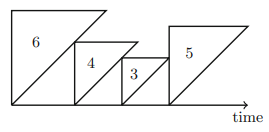
\includegraphics[width=8cm, height=4cm]{primer_trikotnikov.png} 
\end{center}

Trikotniki morajo biti postavljeni tako, da je hipotenuza trikotnika naraščajoča glede na $x$-os, natančneje naklon hipotenuze je enak 1. \\
Želimo si trikotnike postaviti tako, da je dolžina teh trikotnikov najkrajša. Trikotniki se med seboj ne smejo prekrivati,
prav tako pa mora biti krak noge pravokoten na $x$-os.

\subsection{Uporabnost}
Pomembno je, da znamo ta matematični problem interpretirati v praksi. Trikotnike lahko interpretiramo kot opravila na našem urnike. Radi bi minimizirali trajanje našega urnika, medtem ko bi radi prioritizirali bolj kritična oziroma pomembna opravila.
Tako je torej:
\begin{itemize}
    \item pravokotni enakokraki trikotniki $=$ opravila,
    \item dolžina kraka $d_i$ $=$ pomembnost opravila.
\end{itemize}

Želimo si sestaviti urnik iz $n$ opravil. Naj bo $d_i$ pomembnost $i$-tega opravila. Naš cilj je sestaviti čim krajši urnik. Želimo, da se pomembnejša opravila izvedejo, v primeru zakasnitve le teh pa lahko manj pomembna opravila izpustimo.
Večji kot je trikotnik, bolj pomembno je opravilo. Kot je razvidno iz zgornje slike, lahko opravila z manjšo pomembnostjo vstavimo pod opravila z večjo pomembnostjo. To pomeni, da manjše trikotnike vstavljamo pod večje. Torej, če pride do zakasnitve
pomembnejšega opravila (večjega trikotnika), manj pomembno opravilo  izpustimo (manjši trikotnik).


\section{Reševanje problema s pomočjo različnih algoritmov}
V znanstvenem članku The triangle scheduling problem \cite{triangle} je za reševanje problema predlagan Greedy algoritem. Pred Greedy algoritmom sva se odločila sprogramirati brute force algoritem, ki je nekoliko manj težaven, je pa precej časovno zahteven in sicer $O(n!)$. 
Nato sva napisala Greedy algoritem, ki ima nizko časovno zahtevnost vendar ne vrne optimalnega rezultata. Ker Greedy algoritem ne vrne optimuma, sva za konec napisala tudi optimalen algoritem, kjer sva uporabila celoštevilsko linearno programiranje, ki je malo manj časovno zahteven kot brute force. Torej najbolj časovno zahteven algoritem je brute force, takoj za njem pa celoštevilsko linearno programiranje. Najmanj časovno zahteven algoritem je Greedy algoritem, ki rešitev poišče v polinomskem času $O$($n^2$) vendar ne vrne optimalne rešitve. 


\subsection{Brute force algoritem}
\subsubsection{Opis algoritma}
Imamo slovar z n trikotniki in seznam, sestavljen s $n!$ podseznami dolžine n
(vse možne permutacije vrstnega reda trikotnikov). Potem za vsako permutacijo izračuna dolžino urnika in 
dolžine beleži v nov seznam. Ko pregleda vse permutacije, poišče prvo možno permutacijo, ki vrne optimalno rešitev
(minimalno dolžino v seznamu vseh dolžin) in jo vzame za rešitev.

\subsubsection{Psevdokoda}
\begin{verbatim}
    1.     Vhod: trikotniki
    2.     n = length(trikotniki)
    3.     dolzina_urnika = []
    4.     perutacije = permutations( [0, 1, ..., n-1] )
    5.     for i in permutacije
    6.           for j in 0:(n-1)
    7.             trikotnik["vrstni_red"][j] = permutacija[j]
    8.       dolzina_urnika.append( dolzina(trikotniki) )
    9.     index = dolzina_urnika.index( min(dolzina_urnika) )
    10.    for i in 0:(n-1)
    11.      trikotniki[i]["vrstni red"] = permutacije[index][i]
    12.    Izhod: trikotniki

\end{verbatim}




\subsection{Greedy algoritem}
\subsubsection{Opis algoritma}
Greedy algoritem je kateri koli algoritem, ki rešuje problem tako, da na vsakem koraku naredi lokalno optimalno izbiro. Prvi trikotnik razvrsti na $x=0$, kar ustvari prostor pod trikotnikom 1.
Nato vsak trikotnik $j=2,...,n$ postavi na mesto, kjer je dolžina že postavljenih trikotnikov najkrajša. Če je več enakih prostorov, izbere prvega povrsti.
Če ima izbrani prostor pod trikotnikom dolžino $l$ in se začne v času $x_i$, potem je trikotnik $j$ postavljen na mesto $x_j=x_i+d_j$. Če je $2d_j \ge l$,  potem se vsi trikotniki $k$, za katere je $x_k \ge x_j$ zamaknejo za $ 2d_j-l$, da se ne prekrivajo. Opisano 
dogajanje prikazuje spodnji primer, kjer je $x=l$ in $ p_i = d_i $.
\begin{center}
    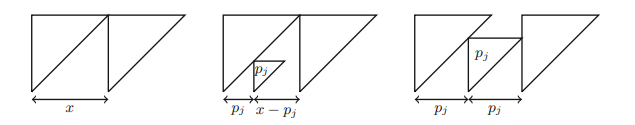
\includegraphics[width=13cm, height=3cm]{greedy.png} 
 \end{center}
Pri številnih problemih Greedy algoritem ne poišče optimalne rešitve in nič drugače ni pri našem problemu.
Na naslednji sliki prikažemo primer, ko Greedy ni optimalen. Greedy algoritem (desna slika) vrne dolzino 42 in ne vrne optimalne dolžine, ki je 40 (leva slika).
\begin{center}
    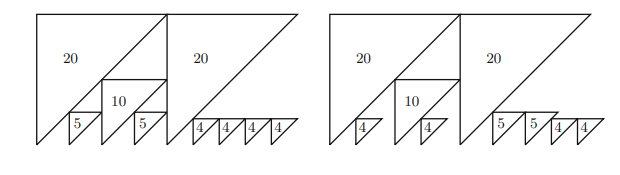
\includegraphics[width=10cm, height=3cm]{primer_neoptimalnosti_greedy.png} 
 \end{center}
Hitrost Greedy algoritma je polinomska. Da se pokazati, da je aproksimacijsko razmerje zgornje meje točnosti Greedy algoritma $1.5$ optimalnega časa. Torej, če je optimalni čas določenega primerna
$40$ časovnih enot, potem Greedy pokaže največ $60$ časovnih enot.

\newpage

\subsubsection{Psevdokoda}
\begin{verbatim}
 Vhod: trikotniki
 n = length(trikotniki)
 trikotniki_lokalno = dict()
 for i in 0:(n-1)
     trikotniki_lokalno[i] = trikotniki[i]
     m = length(trikotniki_lokalno)
     lokalna_dolzina_urnika = []
     for j in 0:(m-1):
         trikotniki_lokalno[i]["vrstni_red"] = j
         *popravi_mesta_ostalim_trikotnikom
         lokalna_dolzina_urnika.append( dolzina_urnika(trikotniki_lokalno) )
     index = lokalna_dolzina_urnika.index( min(lokalna_dolzina_urnika) )
     trikotniki_lokalno[i]["vrstni_red"] = index
     *popravi_mesta_ostalim_trikotnikom
 Izhod: trikotniki_lokalno

\end{verbatim}


Funkcija popravi\_mesta\_ostalim\_trikotnikom nastavi mesta tistih trikotnikov, ki so v slovarju trikotniki\_lokalno, tako da so še vedno urejeni po vrsti in vsak trikotnik ima enolično določeno mesto.
V prvi \texttt{for} for zanki se z vsakim korakom doda nov trikotnik v slovar trikotniki\_lokalno, potem naslednja \texttt{for} zanka pregleda vsa mesta, kamor lahko postavi na novo dodani trikotnik in si dolžine urnika beleži v seznam lokalna\_dolzina\_urnika. Po zaključeni drugi \texttt{for} zanki, se izbere optimalen oziroma najkrajši čas urnika in se za ta določen čas na trikotnike aplicira njihov vrstni red.
Ko se zaključijo vse zanke, imamo v slovarju trikotniki\_lokalno dodane vse vhodne trikotnike, ki so bili postavljeni na lokalno optimalno mesto.


%\subsubsection{Predsatvitev rezultatov}

\subsection{Celoštevilsko linearno programiranje}
V spodnjem primeru privzamemo, da položaj noge oziroma $x$-koordinato označuje $s_i$, $t$ pa označuje dolžino urnika. Spremenljivka $x_{i,j}$ je definirana na naslednji način
$$
x_{i,j} =
\left\{
	\begin{array}{ll}
		1,  & \mbox{če } i\text{-ti trikotnik za} j\text{-tim trikotnikom} \\
		0,  & \mbox{sicer } 
	\end{array}
\right.
$$
in lahko zavzame le vrednosti 0 in 1, medtem ko $s_i$ in $t$ zavzemata pozitivne realne vrednosti. Pogoj $|s_i-s_j| \geq \text{min}\{d_i,d_j\}$ je glavni pogoj v najinem linearnem programu, ostali pogoji pa več ali manj služijo omejevanju spremenljivk.
\newpage
S pogojem $x_{i,j}+x_{j,i}=1$ povemo, da mora veljati, da je $j$-ti trikotnik pred $i$-tim ali pa, da je $i$-ti trikotnik pred $j$-tim.
$T$ označuje $\sum_{i=1}^n d_i$ in se uporabi zato, da v primeru, ko je $s_j < s_i$ pogoji 2 v spodnjem zgledu vseeno veljajo.
Linearni program bi v matematičnem zapisu izgledal tako:
\begin{center}
    min $t$

    p.p.

    1.  $\forall i: 0 \leq s_i \leq t-d_i$

    \medskip

    2.  $\forall i,j \text{ kjer } i\neq j: s_j - s_i \geq \text{max}\{d_i,d_j\}-T\cdot x_{i,j}$
    \medskip

    3.  $\forall i,j \text{ kjer } i\neq j: x_{i,j}+x_{j,i}=1$
\end{center}
\subsubsection{Psevdokoda}
\begin{verbatim}
    1.     Vhod: seznam_dolzin_trikotnikov
    2.     T = sum(seznam_dolzin_trikotnikov)
    3.     t = new_variable()
    4.     s = new_variable()
    5.     x = new_variable(binary = True)
    6.     set_objective(t, maximization = False)
    7.     for i, d in enumerate(seznam_dolzin_trikotnikov)
    8.         add_constraint(s[i] >= 0)
    9.         add_constraint(s[i] + d <= t)
    10.        for j, e in enumerate(seznam_dolzin_trikotnikov[i+1:], i+1):
    11.            m = min(d, e)
    12.            add_constraint(x[i, j]+x[j, i] = 1)
    13.            add_constraint(s[i] - s[j] >= m - T*x[j, i])
    14.            add_constraint(s[j] - s[i] >= m - T*x[i, j])
    15.     Izhod: seznam s
\end{verbatim}

V prvih 6ih vrsticah definiramo spremenljivke in minimizacijsko funkcijo. V \texttt{for} zankah pa podamo vse pogoje.
Izhodni podatek je seznam \texttt{s}, ki vsebuje položaje nog trikotnikov. 

\subsection{Generiranje podatkov}
Pri generiranju podatkov sva potrebovala zgenerirati $n$ dolžin krakov $d_{i}$. Če sva hotela, da je dolžina $d_{i}$
celoštevilska, sva si pomagala s funkcijo \texttt{random.randint}. Če pa sva želela, da je dolžina kraka $d_{i}$ realno število,
pa sva si pomagala s funkcijo \texttt{random.uniform}. Funkcijama je potrebno podati zgornjo in spodnjo mejo, torej interval iz katerega izbira naključne vrednosti.
\newpage
V zgledu na koncu poročila sva za spodnjo mejo izbrala število 1, za
zgornjo mejo pa število 50. 
Funkcija, ki generira podatke ima parametra $a$ in $b$, ki omogočata izbiro katerega koli intervala, tako da velja 
$d_{i} \in [a,b]; \text{ } a, b \in \mathbf{R}^+  \text{ in } a \leq b$. Funkcija, ki generira podatke, dopušča tudi izbiro celoštevilskih podatkov.



\subsection{Predstavitev rezultatov}
Pri prikazu delovanja vseh treh algoritmov si bomo pomagali z zgledom.
Za testno množico sva izbrala 9 enakokrakih trikotnikov z naslednjimi dolžinami.

\begin{verbatim}
    test = naredi_trikotnike(
                9,
                [ 
                44.513033703890834,
                18.613265453372076,
                27.04233495394404,
                29.803779538038164,
                38.01467639495788,
                43.53220098011497,
                13.90897209250403,
                26.415619884578483,
                49.01780933958118
                ]
            )
\end{verbatim}


Rezultati, ki jih vrnejo algoritmi so sestavljeni iz dolžine celotnega urnika in razporeditev le teh. Rezultati
zgleda so sledeči:
\begin{itemize}
    \item Bruteforce algoritem
\end{itemize}    
    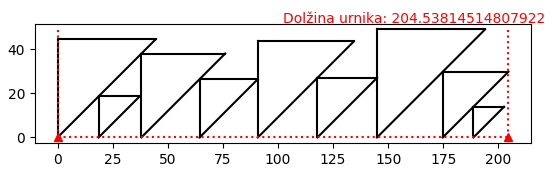
\includegraphics[]{sim_brut.png}
    \newpage
    \begin{itemize}
    \item Celoštevilsko linearno programiranje
\end{itemize}    
    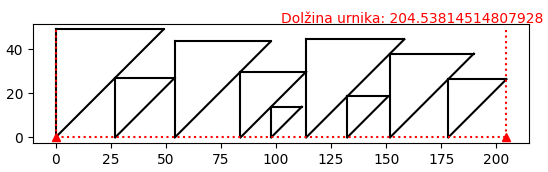
\includegraphics[]{sim_clp.png}
    \begin{itemize}
    \item Greedy algoritem
\end{itemize}    
    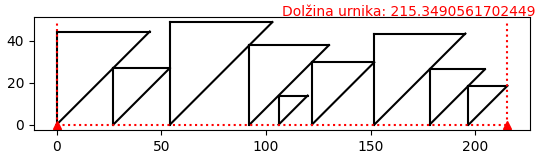
\includegraphics[]{sim_greedy.png}
\\ \\
\textbf{Sklep zgleda}: Opazimo, da tako brute force algoritem in CLP vrneta enako dolžino,
kar se je tudi pričakovalo, saj oba algoritma poiščeta optimalno rešitev. Razlikujeta pa se po
razporeditvi trikotnikov. Pri zgornjem zgledu je 72 različnih razporeditev trikotnikov, ki podajo najmanjšo
razdaljo oz. optimalno rešitev. Z uporabo greedy algoritma pa do optimalne rešitve nismo
prišli. Velikost napake je cca $5,29\%$.

\newpage
\begin{thebibliography}{9}
    \bibitem{triangle}
          Dürr, C., Hanzálek, Z., Konrad, C. et al. The triangle scheduling problem. J Sched 21, 305-312 (2018). \href{https://doi.org/10.1007/s10951-017-0533-1}{https://doi.org/10.1007/s10951-017-0533-1 }
\end{thebibliography}

\end{document}